\documentclass{article}
\usepackage{iclr2027_conference,times}
\usepackage{amsmath,amssymb}
\usepackage{graphicx}
\usepackage{booktabs}
\usepackage{hyperref}

\newcommand{\PhiN}{\Phi}
\newcommand{\phin}{\phi}
\newcommand{\Fw}{F_w}
\newcommand{\Fmu}{F_\mu}
\newcommand{\FC}{F_C}
\newcommand{\FV}{F_V}
\newcommand{\Mm}{\mathcal{M}_\mu}
\newcommand{\MV}{\mathcal{M}_V}
\newcommand{\Rwmu}{R_{w,\mu}}
\newcommand{\Rmuc}{R_{\mu,c}}
\newcommand{\Rcw}{R_{c,w}}
\newcommand{\mout}{\mu_{\mathrm{out}}}
\newcommand{\minn}{\mu_{\mathrm{in}}}

\title{A Gaussian-Kernel Reduction of Small-Uncertainty Discriminatory Learning}

\author{Anonymous authors\\Paper under double-blind review}

\begin{document}
\maketitle

\begin{abstract}
We derive and implement a controlled small-uncertainty reduction of the
microscopic entropic learning dynamics used in the discriminatory society model.
The reduction keeps the original modulation functions, rescales time by the
small uncertainty scale, and averages only over Gaussian issue vectors.  The
result is a set of low-dimensional pairwise kernels depending on ideological
overlap, distrust, and the discrimination field.  We then close these kernels at
the population level using four class/status prototypes and obtain a
semi-analytical phase diagram over discrimination strength \(d\) and
discriminator fraction \(f_d\).  The main signal is affective: the class-trust
order parameter \(\Rmuc\) changes sign with \(d\) and grows in magnitude with
\(f_d\), while the ideological class-alignment order parameter \(\Rcw\) is
essentially constant in this closure.
\end{abstract}

\section{Small-\(C,V\) reduction}

For receiver \(r\), emitter \(e\), and issue vector \(x\), the microscopic
fields are
\begin{equation}
  h_w =
  \frac{\sigma_e \hat w_r^\top x}{\sqrt{1+x^\top C_r x}},
  \qquad
  h_\mu =
  \frac{\mu_{e|r}}{\sqrt{1+V_{e|r}}},
  \qquad
  \sigma_e = \operatorname{sign}(\hat w_e^\top x).
\end{equation}
Discrimination enters by shifting the ideological field,
\(H=h_w+D_{e|r}\).  The evidence and modulation functions are kept exactly as in
the microscopic model:
\begin{align}
  Z(H,\mu) &=
  \PhiN(H)+\PhiN(\mu)-2\PhiN(H)\PhiN(\mu),\\
  \Fw(H,\mu) &=
  \frac{[1-2\PhiN(\mu)]\phin(H)}{Z(H,\mu)},
  &
  \Fmu(H,\mu) &=
  \frac{[1-2\PhiN(H)]\phin(\mu)}{Z(H,\mu)},\\
  \FC(H,\mu) &= -\Fw(H,\mu)[\Fw(H,\mu)+H],
  &
  \FV(H,\mu) &= -\Fmu(H,\mu)[\Fmu(H,\mu)+\mu].
\end{align}
Writing \(C_r=\epsilon \bar C_r\) and \(V_{e|r}=\epsilon \bar V_{e|r}\) with
\(\epsilon\ll1\), the nontrivial limit is obtained on slow time
\(\tau=\epsilon t\).  To leading order,
\begin{align}
  \frac{d\hat w_r}{d\tau}
  &=
  \bar C_r x\sigma_e \Fw(h+D_{e|r},\mu_{e|r}),\\
  \frac{d\mu_{e|r}}{d\tau}
  &=
  \bar V_{e|r}\Fmu(h+D_{e|r},\mu_{e|r}),
\end{align}
where \(h=\sigma_e\hat w_r^\top x\).  The corresponding equations for
\(\bar C_r\) and \(\bar V_{e|r}\) use \(\FC\) and \(\FV\) with the same leading
fields.

\section{Gaussian pairwise kernels}

Let \(u_r=\hat w_r^\top x\) and \(u_e=\hat w_e^\top x\).  For isotropic Gaussian
issues, \((u_r,u_e)\) are jointly Gaussian.  The microscopic ideological field
\(h=\operatorname{sign}(u_e)u_r\) has density
\begin{equation}
  p(h\mid q_r,\rho)
  =
  \frac{2}{\sqrt{q_r}}\,
  \phin\!\left(\frac{h}{\sqrt{q_r}}\right)
  \PhiN\!\left(
  \frac{\rho h}{\sqrt{q_r(1-\rho^2)}}
  \right),
\end{equation}
with separate one-sided limits as \(\rho\to\pm1\).  This gives the affective
kernels
\begin{align}
  \Mm(q_r,\rho,\mu,D)
  &= \int p(h\mid q_r,\rho)\Fmu(h+D,\mu)\,dh,\\
  \MV(q_r,\rho,\mu,D)
  &= \int p(h\mid q_r,\rho)\FV(h+D,\mu)\,dh.
\end{align}
The ideological drift is written as
\begin{equation}
  \mathbb{E}_x[x\,\operatorname{sign}(u_e)\Fw(h+D,\mu)]
  =
  A(q_r,q_e,\rho,\mu,D)\hat w_r
  +
  B(q_r,q_e,\rho,\mu,D)\hat w_e,
\end{equation}
where \(A\) and \(B\) are computed from Gaussian moments.  The implementation
uses Gauss--Hermite quadrature and was checked against direct Monte Carlo
estimates of the original Gaussian issue averages.

\section{Population closure}

To obtain a population-level phase diagram, we group agents into four
prototypes: class A/B crossed with nondiscriminatory/discriminatory receiver
status.  The population weights are
\[
  \frac{1-f_d}{2},\quad \frac{f_d}{2},\quad
  \frac{1-f_d}{2},\quad \frac{f_d}{2}.
\]
For the discriminatory receivers we use the symmetric case-6 field
\[
  D =
  d
  \begin{pmatrix}
  1 & -1\\
  -1 & 1
  \end{pmatrix},
\]
and nondiscriminatory receivers have \(D=0\).  For each ordered prototype pair,
the affective variables evolve according to
\[
  \dot\mu_{e|r}=\bar V_{e|r}\Mm(1,\rho_{re},\mu_{e|r},D_{e|r}),
  \qquad
  \dot{\bar V}_{e|r}=\bar V_{e|r}^{2}\MV(1,\rho_{re},\mu_{e|r},D_{e|r}),
\]
with emitter-rate weights given by the prototype proportions.  Ideological
prototype vectors are evolved using the \(A,B\) drift and then renormalized.

\section{Result}

\begin{figure}[t]
  \centering
  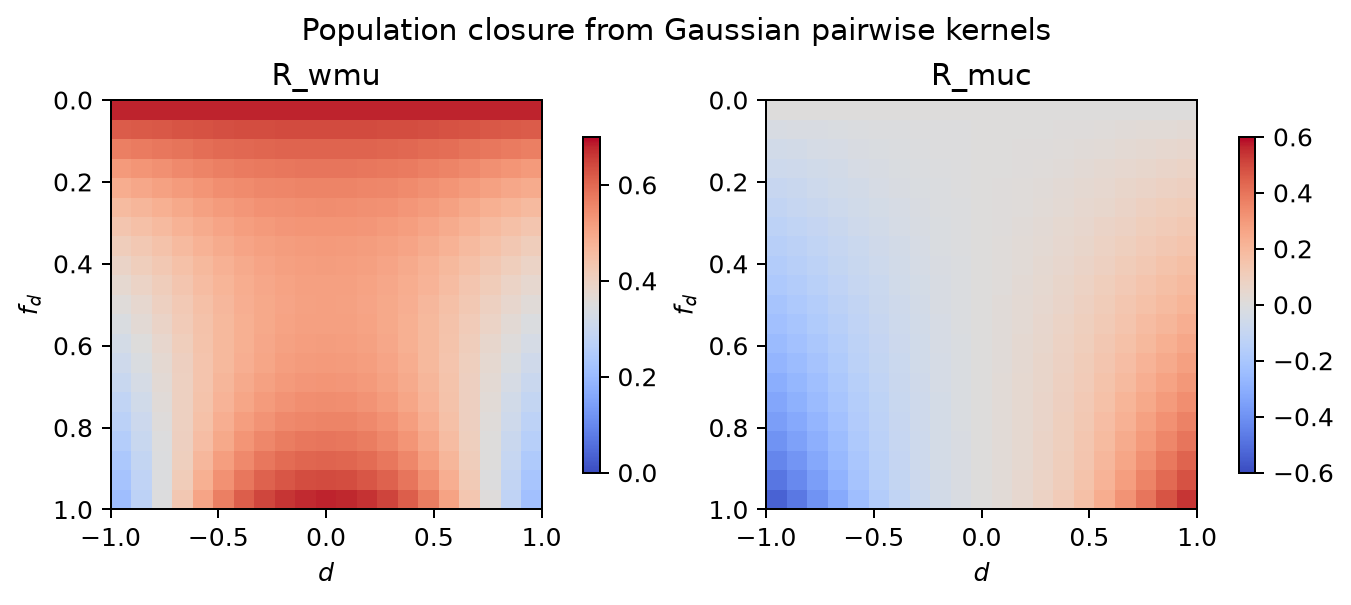
\includegraphics[width=0.92\linewidth]{figures/population_closure_heatmaps_21x21_s240_dt0.05_v1.png}
  \caption{
  Semi-analytical population phase diagram from the Gaussian-kernel closure.
  Left: \(\Rwmu\), plotted on the range \([0,0.7]\).  Right: \(\Rmuc\), plotted
  on the range \([-0.6,0.6]\).  The ideological class-alignment observable
  \(\Rcw\) is not shown because it is nearly constant across this sweep
  (\(\Rcw\simeq 6.3\times10^{-3}\)).
  }
  \label{fig:population-phase}
\end{figure}

Figure~\ref{fig:population-phase} is the main output of the reduction.  The
closure predicts a robust affective ordering: for \(d>0\), discriminatory
receivers become more trusting of their own class and less trusting of the other
class, giving positive \(\Rmuc\); reversing the discrimination field reverses
the sign.  The magnitude of this affective order increases with \(f_d\).  The
mixed trust-ideology observable \(\Rwmu\) remains positive over the full grid and
is largest when the discriminatory fraction is high and \(|d|\) is not too
large.  In contrast, \(\Rcw\) is essentially flat in the present closure.  This
means that the reduced pairwise kernels already capture class-structured trust,
but the current low-rank population closure does not generate a strong
ideological class split.

\section{Stage 4: neutral-state stability}

The rebuild plan calls for a neutral-state stability calculation and, ideally, a
critical curve \(d_c(f_d)\).  We tested this within the four-population closure
by linearizing the affective subsystem around the class-symmetric neutral
configuration.  For \(d\neq0\), however, the neutral state is not an unforced
fixed point: the discrimination field enters the pairwise kernel directly and
creates an additive class-contrast forcing.  Thus the linearized class-contrast
equation has the schematic form
\[
  \frac{d}{d\tau}
  (\mout-\minn)
  =
  J_\mu(\mout-\minn)
  +
  b(f_d,d),
\]
where \(b(f_d,d)\) is nonzero whenever discriminatory receivers are present and
\(d\neq0\).

\begin{figure}[t]
  \centering
  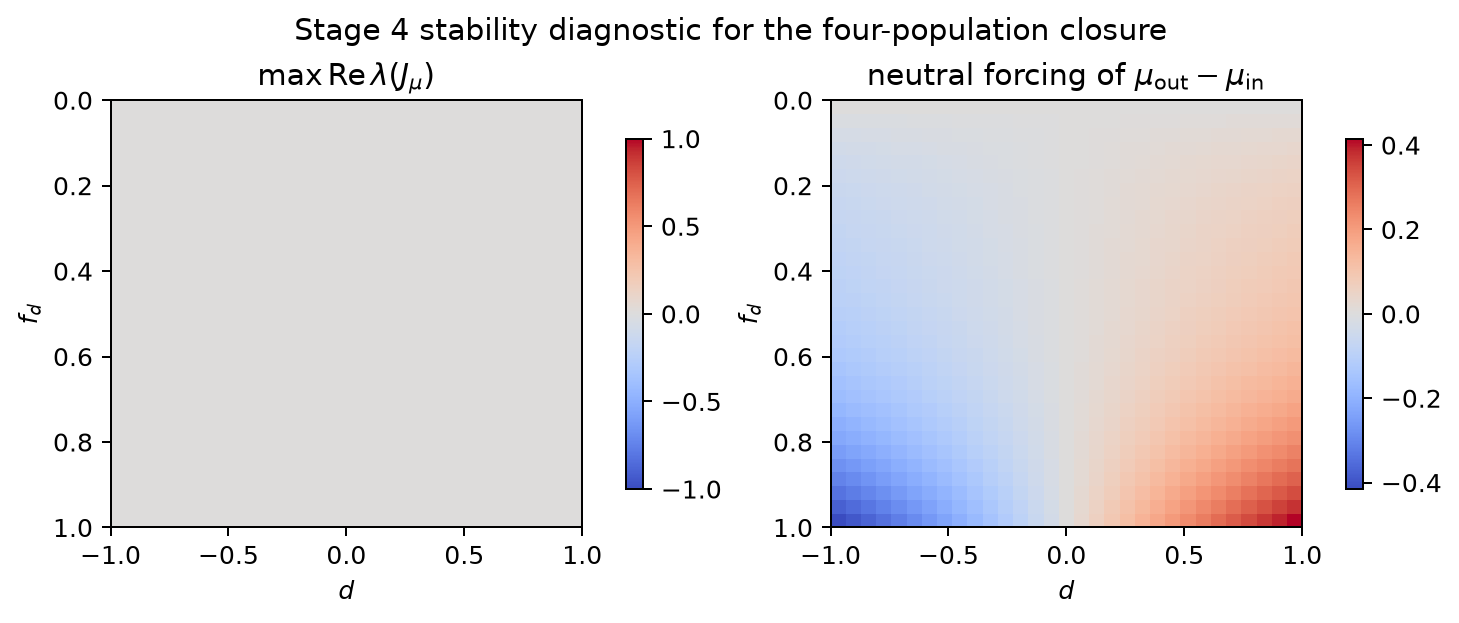
\includegraphics[width=0.92\linewidth]{figures/stage4_neutral_stability_31x31_rho0.98_v1.png}
  \caption{
  Stage-4 diagnostic for the current four-population closure.  Left: the largest
  real eigenvalue of the homogeneous affective block \(J_\mu\), which remains
  zero across the grid.  Right: the direct neutral forcing of the class-trust
  contrast \(\mout-\minn\), which changes sign with \(d\) and grows with
  \(f_d\).  In this closure the class-trust phase diagram is therefore a driven
  response rather than an eigenvalue-crossing instability.
  }
  \label{fig:stage4}
\end{figure}

Figure~\ref{fig:stage4} shows the outcome.  The homogeneous affective block does
not produce a positive eigenvalue or a zero-crossing curve in this approximation.
Instead, the same structure visible in \(\Rmuc\) is already present as a direct
forcing term at the neutral state.  Consequently, this closure does not yet
deliver the desired theoretical transition line \(d_c(f_d)\).  It does identify
the source of the class-trust ordering as the sign-structured pairwise kernel
forcing induced by \(D_{e|r}\).

\section{Two-class attraction boundary}

We also examined a simpler two-class reduction that gives a cleaner analytical
condition for ideological attraction versus repulsion.  Suppose each class is
represented by one normalized prototype vector and let \(\rho\) denote the
cross-class overlap.  For a cross-class interaction, the tangent part of the
ideological drift reduces to
\[
  \dot\rho
  =
  c_{\mathrm{eff}}\,
  B(\rho,\mu_{\mathrm{out}},D_{\mathrm{out}})
  (1-\rho^2),
\]
where \(c_{\mathrm{eff}}>0\) absorbs the interaction rate and the small
uncertainty scale.  Thus the sign of \(B\) determines whether the classes are
locally pulled together or pushed apart in ideology.  Closing the affective
variable by the stationary pairwise condition
\[
  \Mm(\rho,\mu_{\mathrm{out}}^*,-d)=0
\]
gives the candidate boundary
\[
  \boxed{
  B(\rho,\mu_{\mathrm{out}}^*(\rho,d),-d)=0.
  }
\]

\begin{figure}[t]
  \centering
  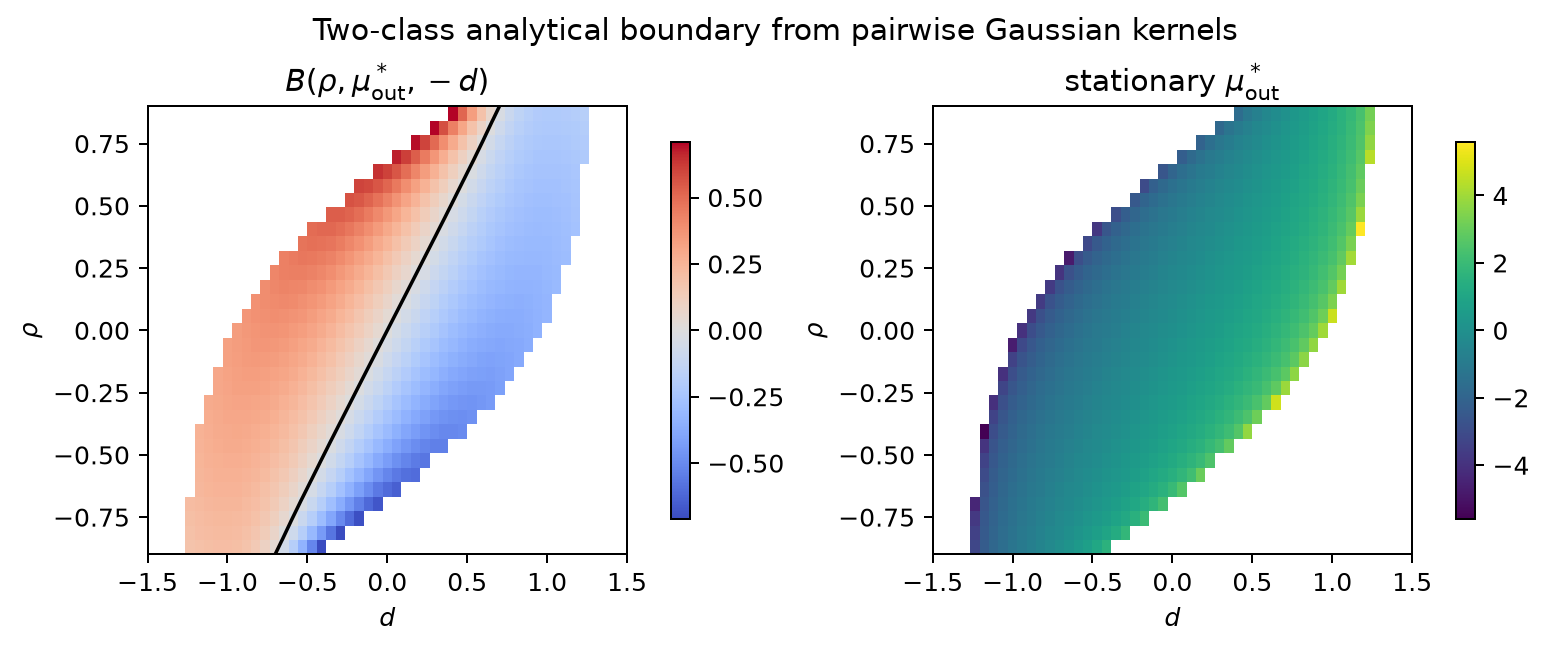
\includegraphics[width=0.92\linewidth]{figures/two_class_boundary_31x51.png}
  \caption{
  Two-class analytical attraction boundary.  The black contour is
  \(B(\rho,\mu_{\mathrm{out}}^*,-d)=0\).  On one side of the contour the
  cross-class ideological drift is attractive, and on the other it is repulsive.
  White regions indicate parameter values where the stationary equation
  \(\Mm=0\) had no finite root in the search window.
  }
  \label{fig:two-class-boundary}
\end{figure}

Figure~\ref{fig:two-class-boundary} is the most promising analytical boundary
obtained so far.  It is not yet the full \(d_c(f_d)\) curve requested by the
rebuild plan because \(f_d\) has been absorbed into the effective interaction
rate in this two-class limit.  Nevertheless, it gives an explicit kernel-level
condition for when the ideological part of the dynamics changes from
cross-class attraction to cross-class repulsion.

\section{Limitations}

This calculation is semi-analytical rather than fully analytical: Gaussian
quadrature is used for the pairwise kernels, and the final population equation is
a four-prototype closure.  The nearly constant \(\Rcw\) should therefore be read
as a limitation of this closure, not as a proof that ideological ordering is
absent in the microscopic model.  A sharper closure should evolve the covariance
kernel \(\bar C_r\) rather than replacing each population by a normalized
prototype vector.  The Stage-4 calculation also shows that this closure does not
yet supply a spontaneous neutral-state instability or a predicted
\(d_c(f_d)\).  Obtaining such a line likely requires a closure in variables
\(\rho_{ab}\), \(\mu_{b|a}\), and anisotropic uncertainty modes, followed by a
Jacobian analysis of a true neutral fixed point.

\end{document}
